\chapter{Sequenzdiagramme}

\begin{figure}[H]
  \centering
  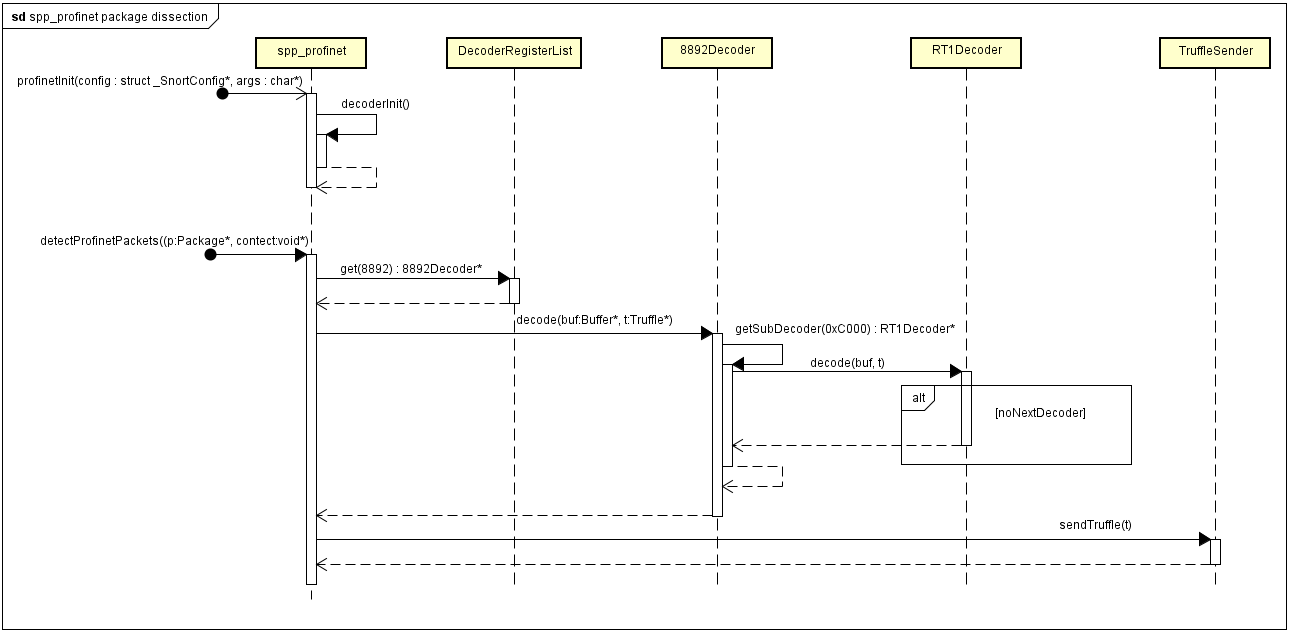
\includegraphics[width=\textwidth]{../diagramimages/spp-profinet-package-dissection.png}
  \caption[Sequenzdiagramm \gls{sppname} package dissection]{Sequenzdiagramm \gls{sppname} package dissection}
\end{figure}

In dieser Sequenz werden zwei zentrale Aufrufe von \gls{snort} im \gls{praeprozessor} \gls{sppname} dargestellt. Zum Einen im oberen Teil die Initialisierung des \gls{praeprozessor}s durch einen Init-Aufruf, sowie der \gls{praeprozessor}-interne Aufbau des DecoderRegisters. Dieser Registrierungsvorgang wurde im Diagramm aus Platzgründen eingespaart. Darin wird jeder als C-Datei vorhandene Decoder instanziiert und bei der DecoderRegisterList registriert. Dieser Vorgang legt die Grundlage für den Decoder-Baum-Ablauf, welcher exemplarisch als zweiter unterer Teil des Sequenzdiagramms modelliert wurde. Für jedes empfangene Paket ruft \gls{snort} die detectProfinetPackets in \sppname auf und übergibt eine Packetpointer. Basierend auf dem Ethertype wählt die DecoderRegisterList den ersten Decoder aus und übergibt den Pointer. \gls{sppname} ruft in diesem Decoder die decode-Methode auf, welche intern basierend auf gefundenen Informationen, sich einen seiner Subdecoder aussucht und in diesem die decode-Methode aufruft. Dieser rekursive Schritt wird solange wiederholt, bis kein Subdecoder mehr vorhanden ist oder das Ende des \gls{paket}s gefunden wurde.
Nach der Rückkehr der Methoden wird das fertige Truffle mit dem TruffleSender in Richtung \gls{programname} per \gls{ipc} verschickt.